\documentclass{beamer}
\usetheme[progressbar=foot]{metropolis}
\usepackage{times}
\usepackage{tikz}
\usepackage{amsmath}
\usepackage{verbatim}
\usepackage{adjustbox}
\usepackage{listings}
\usepackage{verbatim}
\usepackage{array}
\usetikzlibrary{arrows,automata}
\setbeamercolor{progress bar}{fg=red,bg=}
\lstset{language=C,
  basicstyle=\ttfamily,
  keywordstyle=\color{blue}\ttfamily,
  stringstyle=\color{gray}\ttfamily,
  commentstyle=\color{green}\ttfamily,
  morecomment=[l][\color{blue}]{\#}
}

\title{Ghidra\\An Open Source Reverse Engineering Tool}
\date{FrOSCon 2019, 10th August}
\author{Lars A. Wallenborn}
\institute{How the NSA open-sourced all software in 2019}
\begin{document}
\tikzstyle{every picture}+=[remember picture]

  \maketitle
  \section{Intro}
  \begin{frame}{whoami}
    Lars A. Wallenborn\\
    lars@wallenborn.net\\
    @larsborn\\
    \pause
    \vspace{1cm}
    Since 2004 IT Freelancer\\
    2013 Diploma in Mathematics @ Uni Bonn\\
    2014 - 2015 Software Developer in Bonn\\
    Since 2015: Security Researcher at CrowdStrike
  \end{frame}

  \begin{frame}{Overview}
    \begin{enumerate}
      \item What is Reverse Engineering?
      \item Why should I do it?
      \item How do I do it?
    \end{enumerate}
  \end{frame}

  \section{What is Reverse Engineering}
  \begin{frame}{What is Reverse Engineering}
    \begin{itemize}
      \item \emph{RE} or \emph{reversing} for short\pause
      \item very general term: \pause process of "reversing" the production process of an artificial object\pause
      \item with the aim to reveal its designs, architecture, or -- generally -- to extract knowledge
    \end{itemize}
    \pause
    \begin{alertblock}{This Presenation}\pause
      We will focus on a very specific kind of Reverse Engineering:\\
      \begin{center}
        \emph{Binary Software Reverse Engineering}
      \end{center}
    \end{alertblock}
  \end{frame}

  \begin{frame}{Binary Software Reverse Engineering}
    \begin{adjustbox}{max totalsize={.9\textwidth}{.7\textheight},center}
      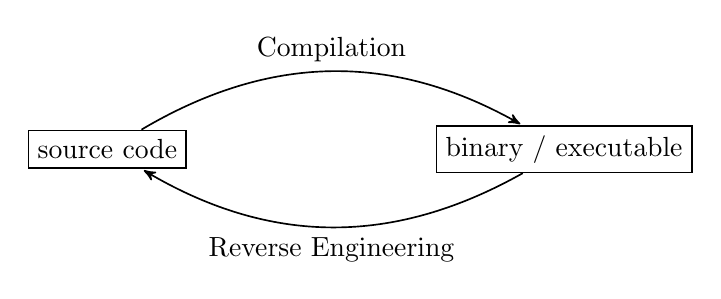
\begin{tikzpicture}[->,>=stealth',shorten >=1pt,auto,node distance=5.8cm,
        semithick]
      \node[rectangle,draw] (A)              {source code};
      \node[rectangle,draw] (B) [right of=A] {binary / executable};

      \path (A) edge[bend left] node {Compilation} (B);
      \pause
      \path (B) edge[bend left] node {Reverse Engineering} (A);
      \end{tikzpicture}
    \end{adjustbox}
  \end{frame}

  \begin{frame}{Binary Software Reverse Engineering -- More General}
    \begin{adjustbox}{max totalsize={.9\textwidth}{.7\textheight},center}
      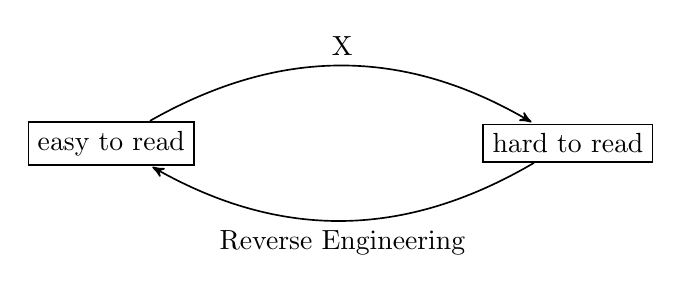
\begin{tikzpicture}[->,>=stealth',shorten >=1pt,auto,node distance=5.8cm,
        semithick]
      \node[rectangle,draw] (A)              {easy to read};
      \node[rectangle,draw] (B) [right of=A] {hard to read};

      \path (A) edge[bend left] node {X} (B);
      \path (B) edge[bend left] node {Reverse Engineering} (A);
      \end{tikzpicture}
    \end{adjustbox}
  \end{frame}

  \section{Why should I do it?}
  \begin{frame}{Motivation}
    \begin{itemize}
      \item Quality Assurance\pause: Does it do what it is supposed to do?\pause
      \item Interoperatibility\pause: A wild undocumented binary blog appears.\pause
      \item Educational Purposes\pause: Excuse to hack.\pause
      \item Malware Analysis\pause: Understand The Bad Guys\texttrademark.\pause
      \item Exploit Development\pause: Are there bugs? Can I exploit them to make it behave in a way it was not intended?\pause
      \item Cracking\pause: How to circumvent copy right protection?\pause
      \item Economic Espionage\pause: How does it work with the goal to reimplement it and then sell it.
    \end{itemize}
    \pause
    \begin{alertblock}{I am not a lawyer}\pause
      But this is roughly sorted by how legal I think it is. \pause In Germany. \pause On a sunny day.
    \end{alertblock}
  \end{frame}

  \section{How do I do it?}
  \begin{frame}[fragile]{Show me an Example!}
    \pause
    \begin{lstlisting}
      #include <stdio.h>

      int main() {
          printf("Hallo FrOSCon!");

          return 0;
      }
  \end{lstlisting}
  \end{frame}

  \begin{frame}[fragile]{Compile it!}
    Compile C program to a binary.
    \begin{verbatim}
      gcc main.c
    \end{verbatim}
    \pause
    \begin{verbatim}
      strip a.exe
    \end{verbatim}
  \end{frame}

  \begin{frame}[fragile]{strings Based Reversing}
    \begin{center}
      Demo
    \end{center}
  \end{frame}

  \begin{frame}[fragile]{What can we deduce already?}
    \pause
    \begin{itemize}
      \item \verb|!This program cannot be run in DOS mode.|\pause\\ $\Rightarrow$ It probably is a Windows executable.\pause
      \item \verb|Hallo FrOSCon!|\pause\\ $\Rightarrow$ suggests that this is a "hello world program".\pause
      \item \verb|Mingw-w64 runtime failure:|\pause\\ $\Rightarrow$ probably compiled with MinGW (Minimalist GNU for Windows).\pause
    \end{itemize}
    \begin{alertblock}{Too many ``probably''s and ``suggests''s?}\pause
      Due to time constraints while reversing, you often have to find a balance between speed and confidence.
    \end{alertblock}
  \end{frame}

  \begin{frame}{Overview}
    \begin{enumerate}
      \item What is Reverse Engineering?
      \item Why should I do it?
      \item How do I do it?
      \pause
      \begin{enumerate}
        \item Static vs. Dynamic Reverse Engineering
        \item Executable Formats
        \item Assembly
        \item Tools
        \item How to get started with Ghidra?
      \end{enumerate}
    \end{enumerate}
  \end{frame}

  \section{Static vs. Dynamic Reverse Engineering}
  \begin{frame}{Static vs. Dynamic Reverse Engineering}\pause
    \begin{alertblock}{Definition: Dynamic Reversing}
      Dynamic software reverse engineering is the analysis of computer software that is performed
      by executing programs on a real or virtual processor.
    \end{alertblock}\pause
    \begin{alertblock}{Definition: Static Reversing}
      Static software reverse engineering is the analysis of computer software that is performed
      without actually executing the target program.
    \end{alertblock}
  \end{frame}

  \section{Executable Formats}
  \begin{frame}{Executable Formats}
    \begin{itemize}
      \item Depends on operating system\pause. We will focus on Windows.\pause
      \item Windows uses the Portable Executable (PE) format.\pause
      \item RE techniques heavily depend on the used programming language. C, C++, Delphi, Go, .NET $\ldots$\pause
      \item Focus on "native" PE files, i.e. files that are "normal" Windows executables.
    \end{itemize}
  \end{frame}

  \begin{frame}[fragile]{PE files}\pause
    \begin{itemize}
      \item PE files contain so-called \emph{sections}.\pause
      \item Named like \verb|.text|, \verb|.data|, \verb|.rdata| or \verb|.bss|.\pause
      \item When the program is executed, the so-called \emph{PE loader} copies the content of these sections
      to different regions in memory.\pause
      \item Then, execution is handed over to the so-called \emph{entry point} within the \verb|.text| section.
    \end{itemize}
  \end{frame}

  \section{Assembly}
  \begin{frame}[fragile]{Assembly}\pause
    \begin{itemize}
      \item Low-Level language executed by the CPU.\pause
      \item Only able to do very basic things.\pause
      \item Central concepts: Registers, Stack, Functions.\pause
      \item Often shown in disassembled state\pause: Instead of
      \begin{verbatim}
        4881ec98000000
      \end{verbatim}
      \pause we see
      \begin{lstlisting}
        SUB RSP, 0x98
      \end{lstlisting}
      \end{itemize}
  \end{frame}

  \section{Tools}
  \begin{frame}{Tools}\pause
    \begin{itemize}
      \item IDA \pause (Interactive Disassembler) \pause + HexRays Decompiler\pause
      \item Binary Ninja\pause
      \item RetDec \pause (retargetable decompiler)\pause
      \item Ghidra
    \end{itemize}
  \end{frame}

  \section{Ghidra}
  \begin{frame}{What is Ghidra?}
    \begin{itemize}
      \item Existence is publicly known since the Vault7 leaks in 2017.\pause
      \item At the RSA security conference 2019, the NSA announced to release it as open source software.\pause
      \item Really did so in the following months.\pause
      \item JAVA-based GUI, backend written in C.\pause
      \item Capable of \pause \emph{decompiling} native PEs\pause
      \item (und many other formats)
    \end{itemize}
  \end{frame}

  \begin{frame}{What can Ghidra do?}\pause
    \begin{itemize}
      \item Import executables and disassemble them\pause
      \item Decompile the assembly and display pseudo code (C-like)\pause
      \item Guess variable and function names when possible\pause
      \item Allow some basic refactoring similar to an integrated development environment (IDE)
    \end{itemize}
  \end{frame}

  \begin{frame}{How do I use it?}
    \begin{center}
      Demo
    \end{center}
  \end{frame}

  \begin{frame}{Thank You}
    Lars A. Wallenborn\\
    lars@wallenborn.net\\
    @larsborn\\
    \vspace{1cm}
    Some advertisement: I will give Reverse Engineering classes soon.
    If you are interested, talk to me or sent me an email!\\
    \pause
    \vspace{1cm}
    Questions?\\
  \end{frame}

  \section{Appendix: Static vs. Dynamic RE Comparison}
  \begin{frame}{Static vs. Dynamic Comparison Comparison}\pause
    \begin{table}
      \begin{tabular}{l|l}
        Static Analyis  & Dynamic Analyis \\
        \hline
        \onslide<3->{timeconsuming} & \onslide<6->{evasion techniques (arms race)}\\
        \onslide<4->{resource intensive (humans)} & \onslide<7->{resource intensive (computers)}\\
        \onslide<5->{not fool-prove} & \onslide<8->{not fool-prove}\\
      \end{tabular}
    \end{table}
    \onslide<9->{
    \begin{alertblock}{Conclusion}
      A combined approach is the best of course.\\
      We will focus on static analysis here.
    \end{alertblock}}
  \end{frame}

  \section{Appendix: Assembly}
  \begin{frame}[fragile]{Assembly: Registers}\pause
    \begin{itemize}
      \item There are around 16 registers in a 64-bit CPU.\pause
      \item Named like \verb|RAX|, \verb|RBP| or \verb|R8|.\pause
      \item Each register can store 64 bit of data.\pause
      \item They are extremly fast (even compared to RAM).\pause
      \item Example:\pause
    \end{itemize}
    \begin{lstlisting}
      MOV RAX, 0x12
      SUB RAX, 0x8
      ADD RAX, 0x4
    \end{lstlisting}\pause
    \begin{itemize}
      \item Each instructions is made up of a \emph{mnemonic} and (optionally) \emph{arguments}.\pause
      \item Depending on how you count there are between 1000 and 4000 assembly instructions.
    \end{itemize}
  \end{frame}

  \begin{frame}[fragile]{Assembly: Instruction Pointer}\pause
    \begin{itemize}
      \item There is a \emph{very} special register: \verb|RIP|.\pause
      \item It stores the address of the next assembly command that should be executed by the CPU.\pause
      \item Yes, the program lives in the same space as the data.\pause
      \item This is the cause of \emph{many} problems we have with computers nowadays.\pause
    \end{itemize}
  \end{frame}

  \begin{frame}[fragile]{Assembly: Stack}\pause
    \begin{itemize}
      \item Central datastructure.\pause
      \item Resides in RAM.\pause
      \item Literally a \emph{stack}.\pause
      \item \verb|PUSH| and \verb|POP| can be used to manipulate it.\pause
      \item Registers \verb|RSP| and \verb|RBP| store its location.\pause
      \item Example:\pause
    \end{itemize}
    \begin{lstlisting}
      PUSH RBX
      PUSH 0x98
      POP RBX
    \end{lstlisting}
  \end{frame}

  \begin{frame}[fragile]{Assembly: Functions}\pause
    \begin{itemize}
      \item Often functions in C are compiled to functions in assembly.\pause
      \item \verb|CALL| and \verb|RET| are the responsible mnemonics.\pause
      \item Example:\pause
    \end{itemize}
    \begin{lstlisting}
      CALL f5 15 00 00
      CALL printf
      RET
    \end{lstlisting}
    \pause
    \begin{itemize}
      \item \verb|CALL| pushes \verb|EIP| to the stack\pause
      \item And then sets its value to the given argument\pause
      \item Effectively continuing execution in the function\pause
      \item \verb|RET| does the inverse.\pause
      \item This allow arbitrarily deeply nested calls.
    \end{itemize}
  \end{frame}

\end{document}
